\documentclass[14pt]{extbook}
\usepackage{multicol, enumerate, enumitem, hyperref, color, soul, setspace, parskip, fancyhdr} %General Packages
\usepackage{amssymb, amsthm, amsmath, latexsym, units, mathtools} %Math Packages
\everymath{\displaystyle} %All math in Display Style
% Packages with additional options
\usepackage[headsep=0.5cm,headheight=12pt, left=1 in,right= 1 in,top= 1 in,bottom= 1 in]{geometry}
\usepackage[usenames,dvipsnames]{xcolor}
\usepackage{dashrule}  % Package to use the command below to create lines between items
\newcommand{\litem}[1]{\item#1\hspace*{-1cm}\rule{\textwidth}{0.4pt}}
\pagestyle{fancy}
\lhead{Progress Quiz 6}
\chead{}
\rhead{Version A}
\lfoot{9689-6866}
\cfoot{}
\rfoot{Spring 2021}
\begin{document}

\begin{enumerate}
\litem{
Determine the horizontal and/or oblique asymptotes in the rational function below.\[ f(x) = \frac{6x^{3} -5 x^{2} -66 x -40}{3x^{2} -10 x -8} \]\begin{enumerate}[label=\Alph*.]
\item \( \text{Horizontal Asymptote of } y = 2.0 \text{ and Oblique Asymptote of } y = 2x + 5 \)
\item \( \text{Oblique Asymptote of } y = 2x + 5. \)
\item \( \text{Horizontal Asymptote of } y = 2.0  \)
\item \( \text{Horizontal Asymptote at } y = 4.0 \)
\item \( \text{Horizontal Asymptote of } y = 4.0 \text{ and Oblique Asymptote of } y = 2x + 5 \)

\end{enumerate} }
\litem{
Which of the following functions \textit{could} be the graph below?
\begin{center}
    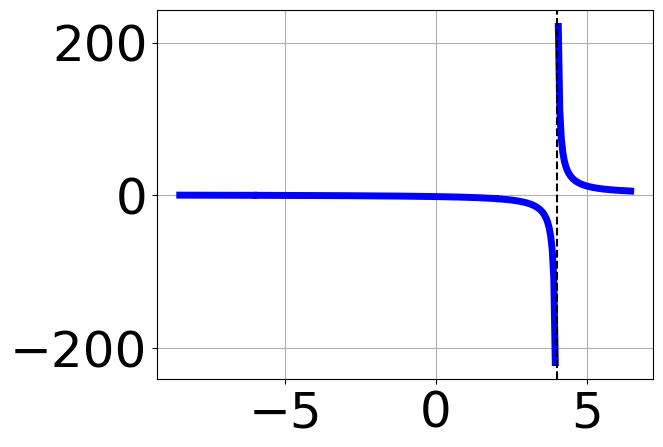
\includegraphics[width=0.5\textwidth]{../Figures/identifyGraphOfRationalFunctionA.png}
\end{center}
\begin{enumerate}[label=\Alph*.]
\item \( f(x)=\frac{x^{3} -7 x^{2} + 36}{x^{3} -2 x^{2} -29 x -42} \)
\item \( f(x)=\frac{x^{3} -7 x^{2} + 36}{x^{3} -2 x^{2} -29 x -42} \)
\item \( f(x)=\frac{x^{3} +7 x^{2} -36}{x^{3} +2 x^{2} -29 x + 42} \)
\item \( f(x)=\frac{x^{3} +11 x^{2} +36 x + 36}{x^{3} +2 x^{2} -29 x + 42} \)
\item \( \text{None of the above are possible equations for the graph.} \)

\end{enumerate} }
\litem{
Determine the horizontal and/or oblique asymptotes in the rational function below.\[ f(x) = \frac{3x^{2} -13 x + 12}{15x^{3} +31 x^{2} -104 x + 48} \]\begin{enumerate}[label=\Alph*.]
\item \( \text{Horizontal Asymptote of } y = 0.200  \)
\item \( \text{Horizontal Asymptote at } y = 3.000 \)
\item \( \text{Horizontal Asymptote of } y = 0.200 \text{ and Oblique Asymptote of } y = 5x + 32 \)
\item \( \text{Horizontal Asymptote of } y = 0 \)
\item \( \text{Oblique Asymptote of } y = 5x + 32. \)

\end{enumerate} }
\litem{
Determine the vertical asymptotes and holes in the rational function below.\[ f(x) = \frac{12x^{3} -67 x^{2} +113 x -60}{12x^{2} -35 x + 25} \]\begin{enumerate}[label=\Alph*.]
\item \( \text{Holes at } x = 1.667 \text{ and } x = 1.25 \text{ with no vertical asymptotes.} \)
\item \( \text{Vertical Asymptote of } x = 1.0 \text{ and hole at } x = 1.25 \)
\item \( \text{Vertical Asymptote of } x = 1.667 \text{ and hole at } x = 1.25 \)
\item \( \text{Vertical Asymptotes of } x = 1.667 \text{ and } x = 1.25 \text{ with no holes.} \)
\item \( \text{Vertical Asymptotes of } x = 1.667 \text{ and } x = 1.333 \text{ with a hole at } x = 1.25 \)

\end{enumerate} }
\litem{
Which of the following functions \textit{could} be the graph below?
\begin{center}
    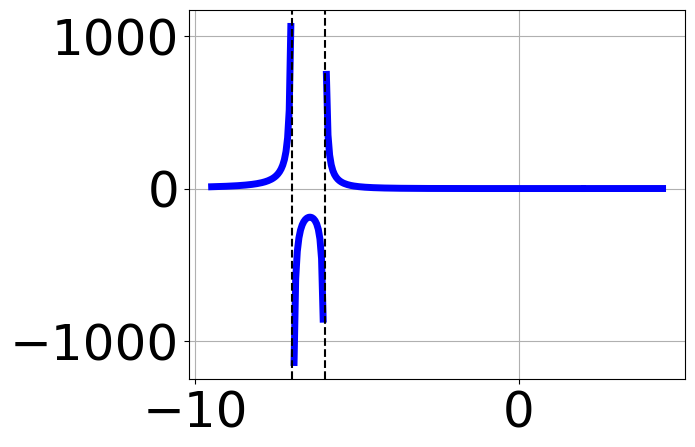
\includegraphics[width=0.5\textwidth]{../Figures/identifyGraphOfRationalFunctionCopyA.png}
\end{center}
\begin{enumerate}[label=\Alph*.]
\item \( f(x)=\frac{x^{3} +3 x^{2} -18 x -40}{x^{3} -7 x^{2} -25 x + 175} \)
\item \( f(x)=\frac{x^{3} -3 x^{2} -18 x + 40}{x^{3} +7 x^{2} -25 x -175} \)
\item \( f(x)=\frac{x^{3} + x^{2} -10 x + 8}{x^{3} +7 x^{2} -25 x -175} \)
\item \( f(x)=\frac{x^{3} +3 x^{2} -18 x -40}{x^{3} -7 x^{2} -25 x + 175} \)
\item \( \text{None of the above are possible equations for the graph.} \)

\end{enumerate} }
\litem{
Determine the vertical asymptotes and holes in the rational function below.\[ f(x) = \frac{16x^{3} -48 x^{2} -9 x + 27}{12x^{2} +25 x + 12} \]\begin{enumerate}[label=\Alph*.]
\item \( \text{Vertical Asymptotes of } x = -1.333 \text{ and } x = -0.75 \text{ with no holes.} \)
\item \( \text{Vertical Asymptote of } x = -1.333 \text{ and hole at } x = -0.75 \)
\item \( \text{Vertical Asymptote of } x = 1.333 \text{ and hole at } x = -0.75 \)
\item \( \text{Vertical Asymptotes of } x = -1.333 \text{ and } x = 0.75 \text{ with a hole at } x = -0.75 \)
\item \( \text{Holes at } x = -1.333 \text{ and } x = -0.75 \text{ with no vertical asymptotes.} \)

\end{enumerate} }
\litem{
Determine the horizontal and/or oblique asymptotes in the rational function below.\[ f(x) = \frac{16x^{3} +8 x^{2} -23 x -15}{4x^{2} -13 x -12} \]\begin{enumerate}[label=\Alph*.]
\item \( \text{Horizontal Asymptote at } y = 4.0 \)
\item \( \text{Horizontal Asymptote of } y = 4.0 \text{ and Oblique Asymptote of } y = 4x + 15 \)
\item \( \text{Horizontal Asymptote of } y = 4.0  \)
\item \( \text{Horizontal Asymptote of } y = 4.0 \text{ and Oblique Asymptote of } y = 4x + 15 \)
\item \( \text{Oblique Asymptote of } y = 4x + 15. \)

\end{enumerate} }
\litem{
Determine the vertical asymptotes and holes in the rational function below.\[ f(x) = \frac{16x^{3} +16 x^{2} -17 x -15}{8x^{2} +22 x + 15} \]\begin{enumerate}[label=\Alph*.]
\item \( \text{Holes at } x = -1.5 \text{ and } x = -1.25 \text{ with no vertical asymptotes.} \)
\item \( \text{Vertical Asymptotes of } x = -1.5 \text{ and } x = -0.75 \text{ with a hole at } x = -1.25 \)
\item \( \text{Vertical Asymptote of } x = 2.0 \text{ and hole at } x = -1.25 \)
\item \( \text{Vertical Asymptotes of } x = -1.5 \text{ and } x = -1.25 \text{ with no holes.} \)
\item \( \text{Vertical Asymptote of } x = -1.5 \text{ and hole at } x = -1.25 \)

\end{enumerate} }
\litem{
Determine the vertical asymptotes and holes in the rational function below.\[ f(x) = \frac{12x^{3} +41 x^{2} -38 x -40}{8x^{2} -22 x + 15} \]\begin{enumerate}[label=\Alph*.]
\item \( \text{Vertical Asymptote of } x = 1.5 \text{ and hole at } x = 1.25 \)
\item \( \text{Vertical Asymptote of } x = 1.5 \text{ and hole at } x = 1.25 \)
\item \( \text{Holes at } x = 1.5 \text{ and } x = 1.25 \text{ with no vertical asymptotes.} \)
\item \( \text{Vertical Asymptotes of } x = 1.5 \text{ and } x = -0.667 \text{ with a hole at } x = 1.25 \)
\item \( \text{Vertical Asymptotes of } x = 1.5 \text{ and } x = 1.25 \text{ with no holes.} \)

\end{enumerate} }
\litem{
Determine the horizontal and/or oblique asymptotes in the rational function below.\[ f(x) = \frac{2x^{2} -7 x + 6}{4x^{3} -8 x^{2} -9 x + 18} \]\begin{enumerate}[label=\Alph*.]
\item \( \text{Oblique Asymptote of } y = 2x + 3. \)
\item \( \text{Horizontal Asymptote of } y = 0 \)
\item \( \text{Horizontal Asymptote at } y = 2.000 \)
\item \( \text{Horizontal Asymptote of } y = 0.500 \text{ and Oblique Asymptote of } y = 2x + 3 \)
\item \( \text{Horizontal Asymptote of } y = 0.500  \)

\end{enumerate} }
\end{enumerate}

\end{document}